%!TEX encoding = UTF-8 Unicode
%!TEX root = ../livre-can.tex

%-----------------------------------------------------------------------------------------------------
%   DESSIN TRAME CAN
%-----------------------------------------------------------------------------------------------------

\newcommand\startcanbit{\pgfmathparse{0}\let\x\pgfmathresult}

\newcommand\cantextstyle{\small\tt}
\newcommand\canbitwidth{.75}
\newcommand\canbitheight{.5}

\newcommand\canbitstyle{[thick, fill=lightgray!25]}

\newcommand\cannobit[1]{
  \pgfmathparse{\x + \canbitwidth * #1}\let\x\pgfmathresult
}
\newcommand\canbit[1]{
  \draw (\x, 0)\canbitstyle rectangle ++ (\canbitwidth, \canbitheight) ;
  \draw (\x + \canbitwidth * 0.5, \canbitheight * 0.5) node {\cantextstyle #1} ;
  \pgfmathparse{\x + \canbitwidth}\let\x\pgfmathresult
}

\newcommand\canbitfield[1]{
  \draw (\x, 0)\canbitstyle rectangle ++ (3 * \canbitwidth, \canbitheight) ;
  \draw (\x + \canbitwidth * 1.5, \canbitheight * 0.5) node {\cantextstyle #1} ;
  \pgfmathparse{\x + 3 * \canbitwidth}\let\x\pgfmathresult
}

\newcommand\canbitl[1]{
  \draw (\x, 0)\canbitstyle -- ++ (0, \canbitheight) ;
  \draw (\x, 0)\canbitstyle -- ++ (\canbitwidth, 0) ;
  \draw (\x + \canbitwidth * 0.5, \canbitheight * 0.5) node {\cantextstyle #1} ;
  \pgfmathparse{\x + \canbitwidth}\let\x\pgfmathresult
  \draw (\x, 0)\canbitstyle -- ++ (0, \canbitheight) ;
}

\newcommand\canbith[1]{
  \draw (\x, 0)\canbitstyle -- ++ (0, \canbitheight) ;
  \draw (\x, \canbitheight)\canbitstyle -- ++ (\canbitwidth, 0) ;
  \draw (\x + \canbitwidth * 0.5, \canbitheight * 0.5) node {\cantextstyle #1} ;
  \pgfmathparse{\x + \canbitwidth}\let\x\pgfmathresult
  \draw (\x, 0)\canbitstyle -- ++ (0, \canbitheight) ;
}

\newcommand\candots{
  \draw (\x, 0)[dotted]\canbitstyle -- ++ (\canbitwidth, 0) ;
  \draw (\x, \canbitheight) [dotted]\canbitstyle -- ++ (\canbitwidth, 0) ;
  \pgfmathparse{\x + \canbitwidth}\let\x\pgfmathresult
}

%-----------------------------------------------------------------------------------------------------

\chapter{Protocole CAN}

%--- Pour supprimer tout en-tête et pied de page sur la 1re page d'un chapitre
\thispagestyle{empty}


\begin{figure}[h!]
  \centering
  \begin{tikzpicture}[transform shape, rotate=90]
    \draw ( 2 * \canbitwidth, 0)[dotted] -- ++ (0, 4) ;
    \draw ( 3 * \canbitwidth, -4.5)[dotted] -- (3 * \canbitwidth, 1.25) ;
    \draw ( 6 * \canbitwidth, -4.5)[dotted] -- ++ (0, 1) ;
    \draw ( 3 * \canbitwidth, -4.5)[<->] -- ++ (3 * \canbitwidth, 0) node[midway, above]{11 bits} ;
    \draw ( 8 * \canbitwidth, -4.5)[dotted] -- ++ (0, 1) ;
    \draw ( 11 * \canbitwidth, -4.5)[dotted] -- ++ (0, 1) ;
    \draw ( 8 * \canbitwidth, -4.5)[<->] -- ++ (3 * \canbitwidth, 0) node[midway, above]{19 bits} ;
    \draw ( 6 * \canbitwidth, 1.25)[dotted] -- ++ (0, -2) -- ++ (\canbitwidth, 0) -- ++ (0, -2) -- ++ (5 * \canbitwidth, 0) -- ++ (0, -1) ;
    \draw ( 9 * \canbitwidth, 1.25)[dotted] -- ++ (0, -2.25) -- ++ (3 * \canbitwidth, 0) -- ++ (0, -1.5) -- ++ (5 * \canbitwidth, 0) -- ++ (0, -1) ;
    \draw (14 * \canbitwidth, -4.5)[dotted] -- ++ (0, 1) ;
    \draw (17 * \canbitwidth, -4.5)[dotted] -- ++ (0, 1) ;
    \draw (14 * \canbitwidth, -4.5)[<->] -- ++ (3 * \canbitwidth, 0) node[midway, above]{4 bits} ;
    \draw (9 * \canbitwidth, -2.5)[dotted] -- ++ (0, 1) ;
    \draw (9 * \canbitwidth, -2.5)[<->] -- ++ (3 * \canbitwidth, 0) node[midway, above]{4 bits} ;
    \draw (9 * \canbitwidth, -.5)[<->] -- ++ (3 * \canbitwidth, 0) node[midway, above]{0 à 8 octets} ;
    \draw (12 * \canbitwidth, -.5)[dotted] -- ++ (0, 1.75) ;
    \draw (15 * \canbitwidth, 0)[dotted] -- ++ (0, -.5) ;
    \draw (12 * \canbitwidth, -.5)[<->] -- ++ (3 * \canbitwidth, 0) node[midway, above]{15 bits} ;
    \draw (16 * \canbitwidth, 0)[dotted] -- ++ (0, 3) ;
    \draw (18 * \canbitwidth, 0)[dotted] -- ++ (0, 1.25) ;
    \draw (21 * \canbitwidth, 0)[dotted] -- ++ (0, 4) ;
    \draw (2 * \canbitwidth, 4)[<->] -- (21 * \canbitwidth, 4) node[midway, above]{DATA FRAME ou REMOTE FRAME} ;
    \draw (2 * \canbitwidth, 3)[<->] -- (16 * \canbitwidth, 3) node[midway, above]{\emph{Champs où le « bit stuffing » est actif}} ;
    \draw (24 * \canbitwidth, 0)[dotted] -- ++ (0, 1.25) ;
    \draw (27 * \canbitwidth, 0)[dotted] -- ++ (0, 4) ;
    \draw (21 * \canbitwidth, 4)[<->] -- (27 * \canbitwidth, 4) node[midway, above]{INTERFRAME SPACE} ;
    \startcanbit
    \candots
    \canbith{1}
    \draw (2.5 * \canbitwidth, 1) node {SOF} ; \canbitl{0}
    \draw (4.5 * \canbitwidth, 1) node {ARBITRATION} ; \canbitfield{}
    \draw (7.5 * \canbitwidth, 1) node {CONTROL} ; \canbitfield{}
    \draw (10.5 * \canbitwidth, 1) node {DATA} ; \canbitfield{}
    \draw (13.5 * \canbitwidth, 1) node {CRC} ; \canbitfield{CRC SEQUENCE}\canbith{1}
    \draw (17 * \canbitwidth, 1) node {ACK} ; \canbit{*} \canbith{1}
    \draw (19.5 * \canbitwidth, 1) node {EOF} ; \canbitfield{7 bits à 1}
    \draw (22.5 * \canbitwidth, 1) node {INTERMISSION} ; \canbitfield{3 bits à 1}
    \draw (25.5 * \canbitwidth, 1) node {IDLE} ; \canbit{1} \canbit{\dots} \canbit{1}
    \draw (27.5 * \canbitwidth, 1) node {SOF} ; \canbit{0}
    \candots
    \begin{scope}[yshift=-2cm] % Standard
      \startcanbit
      \cannobit{3}
      \canbitfield{id10 à id0}
      \canbit{RTR}
      \canbitl{IDE}
      \canbitl{r0}
      \canbitfield{lg3 à lg0}
    \end{scope}
    \begin{scope}[yshift=-4cm]
      \startcanbit
      \cannobit{3}
      \canbitfield{id28 à id18}
      \canbith{SRR}
      \canbith{IDE}
      \canbitfield{id17 à id0}
      \canbit{RTR}
      \canbitl{r1}
      \canbitl{r0}
      \canbitfield{lg3 à lg0}
    \end{scope}
  \end{tikzpicture}
  \caption{Format d'une trame CAN}
  \labelFigure{figureFormatTrameDonnees}
\end{figure}


\section{Les différents types de trame}

La spécification du protocole CAN définit les types suivants de messages :
\begin{itemize}
\item  la trame de données (« DATA FRAME »), qui transporte des données ;
\item  la trame de requête (« REMOTE FRAME »), qui demande la transmission d’une trame de données avec le même identificateur ;
\item  la trame d’erreur (« ERROR FRAME »), transmise par une station qui détecte une erreur ;
\item  la trame de surcharge (« OVERLOAD FRAME »), transmise par une station en surcharge.
\end{itemize}

Les deux premières font l'objet de la section suivante.






\section{Format d'une trame de données et de requête}

Le format de cette trame est décrit par la \refFigure{}{figureFormatTrameDonnees}. La composition et le rôle de chaque champ seront détaillés dans les sections qui suivent. 






\subsection{Champ \emph{début de trame} (« Start of Frame »)}

\begin{figure}[h]
  \centering
  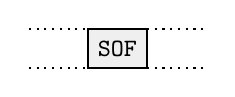
\begin{tikzpicture}
    \startcanbit
    \candots
    \canbit{SOF}
    \candots
  \end{tikzpicture}
  \caption{Début de trame}
  \labelFigure{figureDebutTrame}
\end{figure}

\subsection{Champs \emph{arbitrage} et \emph{contrôle} (« Arbitration Field », « Control Field »)}

Ces deux champs sont décrits simultanément pour être plus facilement compréhensibles. Leur composition est illustrée par la \refFigure{}{figureChampArbitrage}.

\begin{figure}[h]
  \centering
  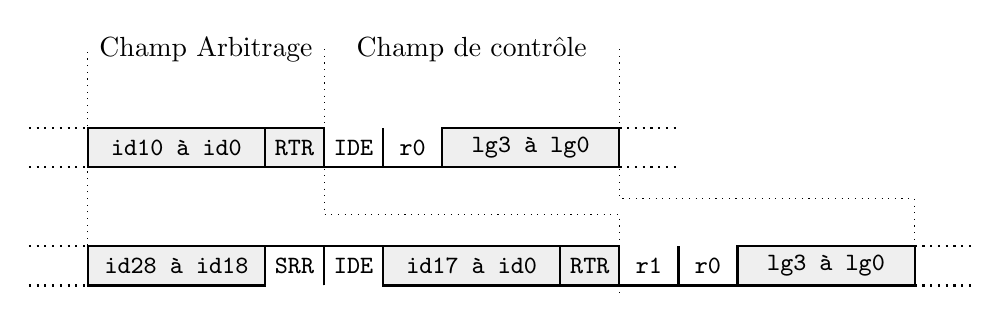
\begin{tikzpicture}
    \draw (\canbitwidth, 0)[dotted] -- ++ (0, 3) ;
    \draw (3 * \canbitwidth, 3) node {Champ Arbitrage} ;
    \draw (7.5 * \canbitwidth, 3) node {Champ de contrôle} ;
    \draw (5 * \canbitwidth, 3)[dotted]
       -- (5 * \canbitwidth, 0.75 + .5 * \canbitheight - 0.1)
       -- ++ (5 * \canbitwidth, 0)
       -- ++ (0, -0.75 - .5 * \canbitheight) ;
    \draw (10 * \canbitwidth, 3)[dotted]
       -- (10 * \canbitwidth, 0.75 + .5 * \canbitheight + 0.1)
       -- ++ (5 * \canbitwidth, 0)
       -- ++ (0, -0.75 - .5 * \canbitheight) ;
    \begin{scope}[yshift=1.5cm]
      \startcanbit
      \candots
      \canbitfield{id10 à id0}
      \canbit{RTR}
      \canbitl{IDE}
      \canbitl{r0}
      \canbitfield{lg3 à lg0}
      \candots
    \end{scope}
    \begin{scope}
      \startcanbit
      \candots
      \canbitfield{id28 à id18}
      \canbith{SRR}
      \canbith{IDE}
      \canbitfield{id17 à id0}
      \canbit{RTR}
      \canbitl{r1}
      \canbitl{r0}
      \canbitfield{lg3 à lg0}
      \candots
    \end{scope}
  \end{tikzpicture}
  \caption{Champ arbitrage et champ de contrôle}
  \labelFigure{figureChampArbitrage}
\end{figure}

\subsection{Champ \emph{de contrôle} (« Control Field »)}


\subsection{Champ \emph{de données} (« Data Field »)}


\subsection{Champ \emph{somme de contrôle} (« Cyclic Redundancy Check Field »)}


\subsection{Champ \emph{d'acquittement} (« Acknowledge Field »)}



\subsection{Fin de la trame (« End of Frame »)}



\subsection{Espace inter-trames (« Interframe Space »)}


\section{Trame d'erreur}





\section{Trame de surchrage}




